\documentclass[1p]{elsarticle_modified}
%\bibliographystyle{elsarticle-num}

%\usepackage[colorlinks]{hyperref}
%\usepackage{abbrmath_seonhwa} %\Abb, \Ascr, \Acal ,\Abf, \Afrak
\usepackage{amsfonts}
\usepackage{amssymb}
\usepackage{amsmath}
\usepackage{amsthm}
\usepackage{scalefnt}
\usepackage{amsbsy}
\usepackage{kotex}
\usepackage{caption}
\usepackage{subfig}
\usepackage{color}
\usepackage{graphicx}
\usepackage{xcolor} %% white, black, red, green, blue, cyan, magenta, yellow
\usepackage{float}
\usepackage{setspace}
\usepackage{hyperref}

\usepackage{tikz}
\usetikzlibrary{arrows}

\usepackage{multirow}
\usepackage{array} % fixed length table
\usepackage{hhline}

%%%%%%%%%%%%%%%%%%%%%
\makeatletter
\renewcommand*\env@matrix[1][\arraystretch]{%
	\edef\arraystretch{#1}%
	\hskip -\arraycolsep
	\let\@ifnextchar\new@ifnextchar
	\array{*\c@MaxMatrixCols c}}
\makeatother %https://tex.stackexchange.com/questions/14071/how-can-i-increase-the-line-spacing-in-a-matrix
%%%%%%%%%%%%%%%

\usepackage[normalem]{ulem}

\newcommand{\msout}[1]{\ifmmode\text{\sout{\ensuremath{#1}}}\else\sout{#1}\fi}
%SOURCE: \msout is \stkout macro in https://tex.stackexchange.com/questions/20609/strikeout-in-math-mode

\newcommand{\cancel}[1]{
	\ifmmode
	{\color{red}\msout{#1}}
	\else
	{\color{red}\sout{#1}}
	\fi
}

\newcommand{\add}[1]{
	{\color{blue}\uwave{#1}}
}

\newcommand{\replace}[2]{
	\ifmmode
	{\color{red}\msout{#1}}{\color{blue}\uwave{#2}}
	\else
	{\color{red}\sout{#1}}{\color{blue}\uwave{#2}}
	\fi
}

\newcommand{\Sol}{\mathcal{S}} %segment
\newcommand{\D}{D} %diagram
\newcommand{\A}{\mathcal{A}} %arc


%%%%%%%%%%%%%%%%%%%%%%%%%%%%%5 test

\def\sl{\operatorname{\textup{SL}}(2,\Cbb)}
\def\psl{\operatorname{\textup{PSL}}(2,\Cbb)}
\def\quan{\mkern 1mu \triangleright \mkern 1mu}

\theoremstyle{definition}
\newtheorem{thm}{Theorem}[section]
\newtheorem{prop}[thm]{Proposition}
\newtheorem{lem}[thm]{Lemma}
\newtheorem{ques}[thm]{Question}
\newtheorem{cor}[thm]{Corollary}
\newtheorem{defn}[thm]{Definition}
\newtheorem{exam}[thm]{Example}
\newtheorem{rmk}[thm]{Remark}
\newtheorem{alg}[thm]{Algorithm}

\newcommand{\I}{\sqrt{-1}}
\begin{document}

%\begin{frontmatter}
%
%\title{Boundary parabolic representations of knots up to 8 crossings}
%
%%% Group authors per affiliation:
%\author{Yunhi Cho} 
%\address{Department of Mathematics, University of Seoul, Seoul, Korea}
%\ead{yhcho@uos.ac.kr}
%
%
%\author{Seonhwa Kim} %\fnref{s_kim}}
%\address{Center for Geometry and Physics, Institute for Basic Science, Pohang, 37673, Korea}
%\ead{ryeona17@ibs.re.kr}
%
%\author{Hyuk Kim}
%\address{Department of Mathematical Sciences, Seoul National University, Seoul 08826, Korea}
%\ead{hyukkim@snu.ac.kr}
%
%\author{Seokbeom Yoon}
%\address{Department of Mathematical Sciences, Seoul National University, Seoul, 08826,  Korea}
%\ead{sbyoon15@snu.ac.kr}
%
%\begin{abstract}
%We find all boundary parabolic representation of knots up to 8 crossings.
%
%\end{abstract}
%\begin{keyword}
%    \MSC[2010] 57M25 
%\end{keyword}
%
%\end{frontmatter}

%\linenumbers
%\tableofcontents
%
\newcommand\colored[1]{\textcolor{white}{\rule[-0.35ex]{0.8em}{1.4ex}}\kern-0.8em\color{red} #1}%
%\newcommand\colored[1]{\textcolor{white}{ #1}\kern-2.17ex	\textcolor{white}{ #1}\kern-1.81ex	\textcolor{white}{ #1}\kern-2.15ex\color{red}#1	}

{\Large $\underline{12n_{0734}~(K12n_{0734})}$}

\setlength{\tabcolsep}{10pt}
\renewcommand{\arraystretch}{1.6}
\vspace{1cm}\begin{tabular}{m{100pt}>{\centering\arraybackslash}m{274pt}}
\multirow{5}{120pt}{
	\centering
	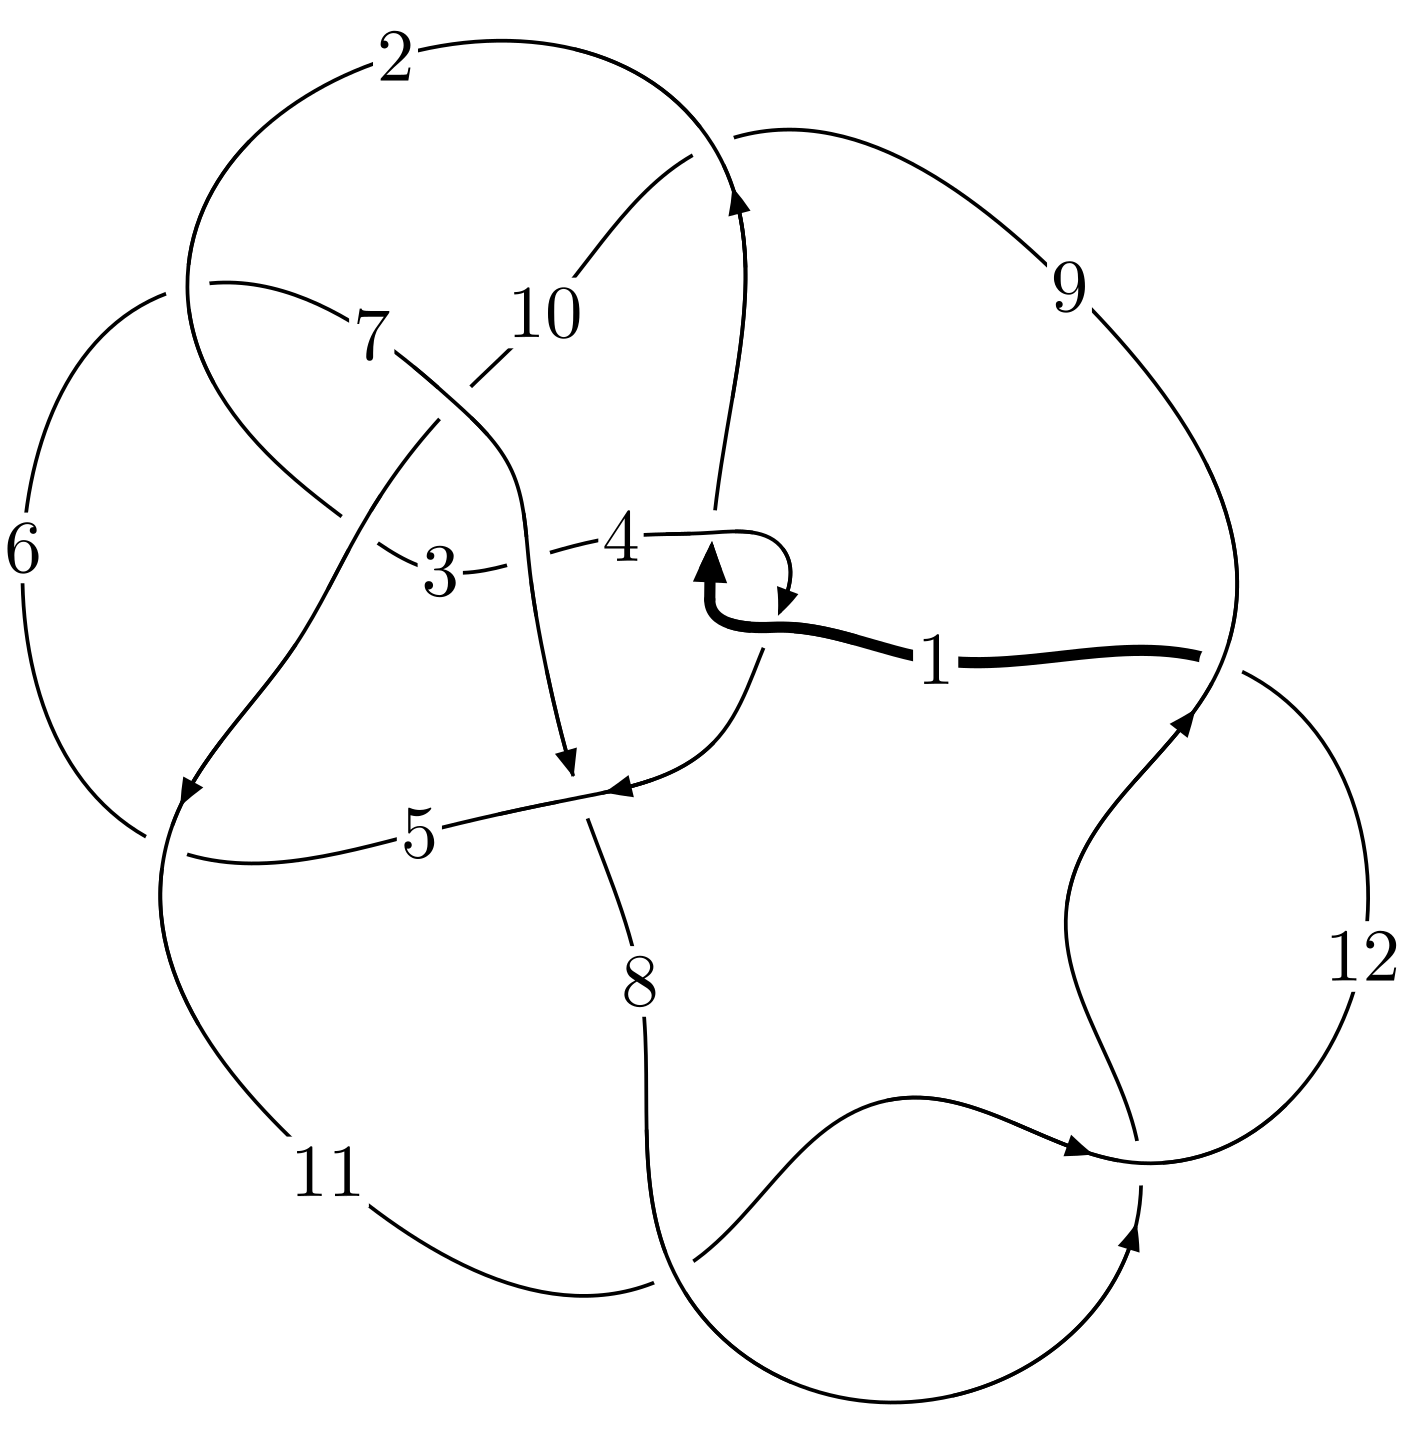
\includegraphics[width=112pt]{../../../GIT/diagram.site/Diagrams/png/2823_12n_0734.png}\\
\ \ \ A knot diagram\footnotemark}&
\allowdisplaybreaks
\textbf{Linearized knot diagam} \\
\cline{2-2}
 &
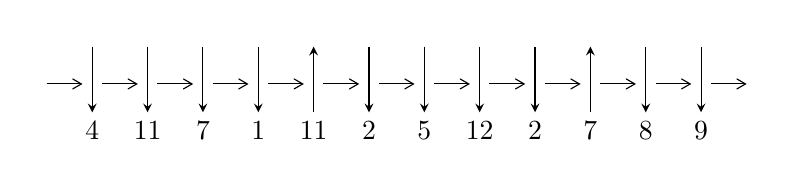
\begin{tikzpicture}[x=20pt, y=17pt]
	% nodes
	\node (C0) at (0, 0) {};
	\node (C1) at (1, 0) {};
	\node (C1U) at (1, +1) {};
	\node (C1D) at (1, -1) {4};

	\node (C2) at (2, 0) {};
	\node (C2U) at (2, +1) {};
	\node (C2D) at (2, -1) {11};

	\node (C3) at (3, 0) {};
	\node (C3U) at (3, +1) {};
	\node (C3D) at (3, -1) {7};

	\node (C4) at (4, 0) {};
	\node (C4U) at (4, +1) {};
	\node (C4D) at (4, -1) {1};

	\node (C5) at (5, 0) {};
	\node (C5U) at (5, +1) {};
	\node (C5D) at (5, -1) {11};

	\node (C6) at (6, 0) {};
	\node (C6U) at (6, +1) {};
	\node (C6D) at (6, -1) {2};

	\node (C7) at (7, 0) {};
	\node (C7U) at (7, +1) {};
	\node (C7D) at (7, -1) {5};

	\node (C8) at (8, 0) {};
	\node (C8U) at (8, +1) {};
	\node (C8D) at (8, -1) {12};

	\node (C9) at (9, 0) {};
	\node (C9U) at (9, +1) {};
	\node (C9D) at (9, -1) {2};

	\node (C10) at (10, 0) {};
	\node (C10U) at (10, +1) {};
	\node (C10D) at (10, -1) {7};

	\node (C11) at (11, 0) {};
	\node (C11U) at (11, +1) {};
	\node (C11D) at (11, -1) {8};

	\node (C12) at (12, 0) {};
	\node (C12U) at (12, +1) {};
	\node (C12D) at (12, -1) {9};
	\node (C13) at (13, 0) {};

	% arrows
	\draw[->,>={angle 60}]
	(C0) edge (C1) (C1) edge (C2) (C2) edge (C3) (C3) edge (C4) (C4) edge (C5) (C5) edge (C6) (C6) edge (C7) (C7) edge (C8) (C8) edge (C9) (C9) edge (C10) (C10) edge (C11) (C11) edge (C12) (C12) edge (C13) ;	\draw[->,>=stealth]
	(C1U) edge (C1D) (C2U) edge (C2D) (C3U) edge (C3D) (C4U) edge (C4D) (C5D) edge (C5U) (C6U) edge (C6D) (C7U) edge (C7D) (C8U) edge (C8D) (C9U) edge (C9D) (C10D) edge (C10U) (C11U) edge (C11D) (C12U) edge (C12D) ;
	\end{tikzpicture} \\
\hhline{~~} \\& 
\textbf{Solving Sequence} \\ \cline{2-2} 
 &
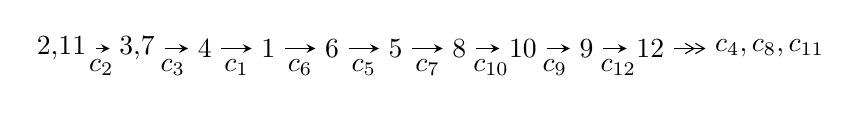
\begin{tikzpicture}[x=23pt, y=7pt]
	% node
	\node (A0) at (-1/8, 0) {2,11};
	\node (A1) at (17/16, 0) {3,7};
	\node (A2) at (17/8, 0) {4};
	\node (A3) at (25/8, 0) {1};
	\node (A4) at (33/8, 0) {6};
	\node (A5) at (41/8, 0) {5};
	\node (A6) at (49/8, 0) {8};
	\node (A7) at (57/8, 0) {10};
	\node (A8) at (65/8, 0) {9};
	\node (A9) at (73/8, 0) {12};
	\node (C1) at (1/2, -1) {$c_{2}$};
	\node (C2) at (13/8, -1) {$c_{3}$};
	\node (C3) at (21/8, -1) {$c_{1}$};
	\node (C4) at (29/8, -1) {$c_{6}$};
	\node (C5) at (37/8, -1) {$c_{5}$};
	\node (C6) at (45/8, -1) {$c_{7}$};
	\node (C7) at (53/8, -1) {$c_{10}$};
	\node (C8) at (61/8, -1) {$c_{9}$};
	\node (C9) at (69/8, -1) {$c_{12}$};
	\node (A10) at (11, 0) {$c_{4},c_{8},c_{11}$};

	% edge
	\draw[->,>=stealth]	
	(A0) edge (A1) (A1) edge (A2) (A2) edge (A3) (A3) edge (A4) (A4) edge (A5) (A5) edge (A6) (A6) edge (A7) (A7) edge (A8) (A8) edge (A9) ;
	\draw[->>,>={angle 60}]	
	(A9) edge (A10);
\end{tikzpicture} \\ 

\end{tabular} \\

\footnotetext{
The image of knot diagram is generated by the software ``\textbf{Draw programme}" developed by Andrew Bartholomew(\url{http://www.layer8.co.uk/maths/draw/index.htm\#Running-draw}), where we modified some parts for our purpose(\url{https://github.com/CATsTAILs/LinksPainter}).
}\phantom \\ \newline 
\centering \textbf{Ideals for irreducible components\footnotemark of $X_{\text{par}}$} 
 
\begin{align*}
I^u_{1}&=\langle 
5.93981\times10^{179} u^{58}+4.60320\times10^{178} u^{57}+\cdots+2.85555\times10^{182} b+1.72195\times10^{182},\\
\phantom{I^u_{1}}&\phantom{= \langle  }8.20063\times10^{181} u^{58}+3.02434\times10^{181} u^{57}+\cdots+1.74189\times10^{184} a-1.14409\times10^{185},\\
\phantom{I^u_{1}}&\phantom{= \langle  }u^{59}+u^{58}+\cdots+386 u+244\rangle \\
I^u_{2}&=\langle 
-659021 u^{16}-928037 u^{15}+\cdots+963035 b-442908,\\
\phantom{I^u_{2}}&\phantom{= \langle  }-299324 u^{16}-63918 u^{15}+\cdots+963035 a-1083657,\;u^{17}+4 u^{15}+\cdots+2 u-1\rangle \\
\\
\end{align*}
\raggedright * 2 irreducible components of $\dim_{\mathbb{C}}=0$, with total 76 representations.\\
\footnotetext{All coefficients of polynomials are rational numbers. But the coefficients are sometimes approximated in decimal forms when there is not enough margin.}
\newpage
\renewcommand{\arraystretch}{1}
\centering \section*{I. $I^u_{1}= \langle 5.94\times10^{179} u^{58}+4.60\times10^{178} u^{57}+\cdots+2.86\times10^{182} b+1.72\times10^{182},\;8.20\times10^{181} u^{58}+3.02\times10^{181} u^{57}+\cdots+1.74\times10^{184} a-1.14\times10^{185},\;u^{59}+u^{58}+\cdots+386 u+244 \rangle$}
\flushleft \textbf{(i) Arc colorings}\\
\begin{tabular}{m{7pt} m{180pt} m{7pt} m{180pt} }
\flushright $a_{2}=$&$\begin{pmatrix}1\\0\end{pmatrix}$ \\
\flushright $a_{11}=$&$\begin{pmatrix}0\\u\end{pmatrix}$ \\
\flushright $a_{3}=$&$\begin{pmatrix}1\\u^2\end{pmatrix}$ \\
\flushright $a_{7}=$&$\begin{pmatrix}-0.00470791 u^{58}-0.00173624 u^{57}+\cdots+17.8688 u+6.56814\\-0.00208009 u^{58}-0.000161202 u^{57}+\cdots+5.50343 u-0.603017\end{pmatrix}$ \\
\flushright $a_{4}=$&$\begin{pmatrix}0.00503808 u^{58}+0.00882567 u^{57}+\cdots+27.3491 u+5.92936\\0.00537009 u^{58}+0.00348580 u^{57}+\cdots+2.87966 u+2.25203\end{pmatrix}$ \\
\flushright $a_{1}=$&$\begin{pmatrix}-0.00261013 u^{58}-0.00116710 u^{57}+\cdots+12.3671 u+6.44607\\0.000615613 u^{58}+0.00164482 u^{57}+\cdots+1.81783 u+0.0786874\end{pmatrix}$ \\
\flushright $a_{6}=$&$\begin{pmatrix}-0.00678800 u^{58}-0.00189745 u^{57}+\cdots+23.3723 u+5.96512\\-0.00208009 u^{58}-0.000161202 u^{57}+\cdots+5.50343 u-0.603017\end{pmatrix}$ \\
\flushright $a_{5}=$&$\begin{pmatrix}-0.00678800 u^{58}-0.00189745 u^{57}+\cdots+23.3723 u+5.96512\\-0.00278773 u^{58}-0.000245605 u^{57}+\cdots+5.27195 u-1.79631\end{pmatrix}$ \\
\flushright $a_{8}=$&$\begin{pmatrix}-0.00902786 u^{58}-0.0115764 u^{57}+\cdots-31.0968 u-6.01473\\-0.00179571 u^{58}-0.00195730 u^{57}+\cdots+3.71563 u+2.05425\end{pmatrix}$ \\
\flushright $a_{10}=$&$\begin{pmatrix}-0.00972417 u^{58}-0.0103974 u^{57}+\cdots-24.0644 u-0.306697\\-0.00277555 u^{58}-0.00259612 u^{57}+\cdots+0.647903 u+1.39356\end{pmatrix}$ \\
\flushright $a_{9}=$&$\begin{pmatrix}-0.0124997 u^{58}-0.0129935 u^{57}+\cdots-23.4165 u+1.08686\\-0.00277555 u^{58}-0.00259612 u^{57}+\cdots+0.647903 u+1.39356\end{pmatrix}$ \\
\flushright $a_{12}=$&$\begin{pmatrix}0.0159522 u^{58}+0.0183199 u^{57}+\cdots+42.8385 u+5.19776\\0.00330850 u^{58}+0.00353952 u^{57}+\cdots-2.63085 u-2.59425\end{pmatrix}$\\&\end{tabular}
\flushleft \textbf{(ii) Obstruction class $= -1$}\\~\\
\flushleft \textbf{(iii) Cusp Shapes $= 0.0183261 u^{58}+0.0259595 u^{57}+\cdots+60.0353 u+1.14679$}\\~\\
\newpage\renewcommand{\arraystretch}{1}
\flushleft \textbf{(iv) u-Polynomials at the component}\newline \\
\begin{tabular}{m{50pt}|m{274pt}}
Crossings & \hspace{64pt}u-Polynomials at each crossing \\
\hline $$\begin{aligned}c_{1},c_{4}\end{aligned}$$&$\begin{aligned}
&u^{59}-6 u^{58}+\cdots-493 u+47
\end{aligned}$\\
\hline $$\begin{aligned}c_{2}\end{aligned}$$&$\begin{aligned}
&u^{59}+u^{58}+\cdots+386 u+244
\end{aligned}$\\
\hline $$\begin{aligned}c_{3}\end{aligned}$$&$\begin{aligned}
&u^{59}-2 u^{58}+\cdots+1473477 u+77047
\end{aligned}$\\
\hline $$\begin{aligned}c_{5}\end{aligned}$$&$\begin{aligned}
&u^{59}-7 u^{57}+\cdots-2336 u+439
\end{aligned}$\\
\hline $$\begin{aligned}c_{6}\end{aligned}$$&$\begin{aligned}
&u^{59}-2 u^{58}+\cdots-4481 u+1539
\end{aligned}$\\
\hline $$\begin{aligned}c_{7}\end{aligned}$$&$\begin{aligned}
&u^{59}-15 u^{58}+\cdots+72 u-4
\end{aligned}$\\
\hline $$\begin{aligned}c_{8},c_{11},c_{12}\end{aligned}$$&$\begin{aligned}
&u^{59}+6 u^{58}+\cdots+2 u+1
\end{aligned}$\\
\hline $$\begin{aligned}c_{9}\end{aligned}$$&$\begin{aligned}
&u^{59}-2 u^{58}+\cdots+2746719 u+257651
\end{aligned}$\\
\hline $$\begin{aligned}c_{10}\end{aligned}$$&$\begin{aligned}
&u^{59}+2 u^{58}+\cdots-394 u+149
\end{aligned}$\\
\hline
\end{tabular}\\~\\
\newpage\renewcommand{\arraystretch}{1}
\flushleft \textbf{(v) Riley Polynomials at the component}\newline \\
\begin{tabular}{m{50pt}|m{274pt}}
Crossings & \hspace{64pt}Riley Polynomials at each crossing \\
\hline $$\begin{aligned}c_{1},c_{4}\end{aligned}$$&$\begin{aligned}
&y^{59}+40 y^{58}+\cdots-8213 y-2209
\end{aligned}$\\
\hline $$\begin{aligned}c_{2}\end{aligned}$$&$\begin{aligned}
&y^{59}+73 y^{58}+\cdots-1655140 y-59536
\end{aligned}$\\
\hline $$\begin{aligned}c_{3}\end{aligned}$$&$\begin{aligned}
&y^{59}+38 y^{58}+\cdots+2137083856067 y-5936240209
\end{aligned}$\\
\hline $$\begin{aligned}c_{5}\end{aligned}$$&$\begin{aligned}
&y^{59}-14 y^{58}+\cdots+6258510 y-192721
\end{aligned}$\\
\hline $$\begin{aligned}c_{6}\end{aligned}$$&$\begin{aligned}
&y^{59}+76 y^{58}+\cdots+38959813 y-2368521
\end{aligned}$\\
\hline $$\begin{aligned}c_{7}\end{aligned}$$&$\begin{aligned}
&y^{59}- y^{58}+\cdots+1240 y-16
\end{aligned}$\\
\hline $$\begin{aligned}c_{8},c_{11},c_{12}\end{aligned}$$&$\begin{aligned}
&y^{59}-58 y^{58}+\cdots-112 y-1
\end{aligned}$\\
\hline $$\begin{aligned}c_{9}\end{aligned}$$&$\begin{aligned}
&y^{59}+44 y^{58}+\cdots-140722482637 y-66384037801
\end{aligned}$\\
\hline $$\begin{aligned}c_{10}\end{aligned}$$&$\begin{aligned}
&y^{59}-82 y^{58}+\cdots+910368 y-22201
\end{aligned}$\\
\hline
\end{tabular}\\~\\
\newpage\flushleft \textbf{(vi) Complex Volumes and Cusp Shapes}
$$\begin{array}{c|c|c}  
\text{Solutions to }I^u_{1}& \I (\text{vol} + \sqrt{-1}CS) & \text{Cusp shape}\\
 \hline 
\begin{aligned}
u &= \phantom{-}0.688572 + 0.799657 I \\
a &= \phantom{-}0.403897 - 0.429993 I \\
b &= \phantom{-}1.319730 + 0.029746 I\end{aligned}
 & -5.51450 + 1.11046 I & -8.00000 + 0. I\phantom{ +0.000000I} \\ \hline\begin{aligned}
u &= \phantom{-}0.688572 - 0.799657 I \\
a &= \phantom{-}0.403897 + 0.429993 I \\
b &= \phantom{-}1.319730 - 0.029746 I\end{aligned}
 & -5.51450 - 1.11046 I & -8.00000 + 0. I\phantom{ +0.000000I} \\ \hline\begin{aligned}
u &= -0.458695 + 0.730749 I \\
a &= \phantom{-}0.541463 + 0.804889 I \\
b &= -0.180739 + 0.082078 I\end{aligned}
 & -1.92960 - 1.37995 I & -8.00000 + 0. I\phantom{ +0.000000I} \\ \hline\begin{aligned}
u &= -0.458695 - 0.730749 I \\
a &= \phantom{-}0.541463 - 0.804889 I \\
b &= -0.180739 - 0.082078 I\end{aligned}
 & -1.92960 + 1.37995 I & -8.00000 + 0. I\phantom{ +0.000000I} \\ \hline\begin{aligned}
u &= -0.263108 + 0.751221 I \\
a &= \phantom{-}0.543851 - 0.807976 I \\
b &= -1.51685 - 0.53259 I\end{aligned}
 & -2.99977 - 6.73475 I & -8.47764 + 5.04092 I \\ \hline\begin{aligned}
u &= -0.263108 - 0.751221 I \\
a &= \phantom{-}0.543851 + 0.807976 I \\
b &= -1.51685 + 0.53259 I\end{aligned}
 & -2.99977 + 6.73475 I & -8.47764 - 5.04092 I \\ \hline\begin{aligned}
u &= \phantom{-}1.248950 + 0.106397 I \\
a &= \phantom{-}0.205733 - 0.100828 I \\
b &= \phantom{-}0.629743 - 0.803792 I\end{aligned}
 & -6.50171 - 1.29569 I & \phantom{-0.000000 } 0 \\ \hline\begin{aligned}
u &= \phantom{-}1.248950 - 0.106397 I \\
a &= \phantom{-}0.205733 + 0.100828 I \\
b &= \phantom{-}0.629743 + 0.803792 I\end{aligned}
 & -6.50171 + 1.29569 I & \phantom{-0.000000 } 0 \\ \hline\begin{aligned}
u &= -0.739660\phantom{ +0.000000I} \\
a &= \phantom{-}0.474782\phantom{ +0.000000I} \\
b &= \phantom{-}0.311743\phantom{ +0.000000I}\end{aligned}
 & -0.974720\phantom{ +0.000000I} & -8.42250\phantom{ +0.000000I} \\ \hline\begin{aligned}
u &= \phantom{-}0.839226 + 1.015310 I \\
a &= \phantom{-}0.149446 + 1.228250 I \\
b &= \phantom{-}0.449432 - 0.919016 I\end{aligned}
 & -0.28824 + 3.32242 I & \phantom{-0.000000 } 0\\
 \hline 
 \end{array}$$\newpage$$\begin{array}{c|c|c}  
\text{Solutions to }I^u_{1}& \I (\text{vol} + \sqrt{-1}CS) & \text{Cusp shape}\\
 \hline 
\begin{aligned}
u &= \phantom{-}0.839226 - 1.015310 I \\
a &= \phantom{-}0.149446 - 1.228250 I \\
b &= \phantom{-}0.449432 + 0.919016 I\end{aligned}
 & -0.28824 - 3.32242 I & \phantom{-0.000000 } 0 \\ \hline\begin{aligned}
u &= -0.621367 + 0.148005 I \\
a &= -1.42430 + 1.76510 I \\
b &= \phantom{-}0.411559 - 0.511446 I\end{aligned}
 & \phantom{-}1.67239 - 2.74169 I & -5.07241 + 2.45099 I \\ \hline\begin{aligned}
u &= -0.621367 - 0.148005 I \\
a &= -1.42430 - 1.76510 I \\
b &= \phantom{-}0.411559 + 0.511446 I\end{aligned}
 & \phantom{-}1.67239 + 2.74169 I & -5.07241 - 2.45099 I \\ \hline\begin{aligned}
u &= \phantom{-}0.087984 + 1.365300 I \\
a &= -0.68821 + 1.42066 I \\
b &= \phantom{-}0.72763 - 1.73513 I\end{aligned}
 & \phantom{-}4.68182 + 3.93350 I & \phantom{-0.000000 } 0 \\ \hline\begin{aligned}
u &= \phantom{-}0.087984 - 1.365300 I \\
a &= -0.68821 - 1.42066 I \\
b &= \phantom{-}0.72763 + 1.73513 I\end{aligned}
 & \phantom{-}4.68182 - 3.93350 I & \phantom{-0.000000 } 0 \\ \hline\begin{aligned}
u &= -0.581835 + 0.198470 I \\
a &= \phantom{-}0.560192 + 0.121209 I \\
b &= \phantom{-}0.808875 + 0.059387 I\end{aligned}
 & -1.109630 - 0.030440 I & -3.69972 - 2.46994 I \\ \hline\begin{aligned}
u &= -0.581835 - 0.198470 I \\
a &= \phantom{-}0.560192 - 0.121209 I \\
b &= \phantom{-}0.808875 - 0.059387 I\end{aligned}
 & -1.109630 + 0.030440 I & -3.69972 + 2.46994 I \\ \hline\begin{aligned}
u &= \phantom{-}1.233130 + 0.644677 I \\
a &= -0.214064 - 0.343399 I \\
b &= -0.159650 + 0.596710 I\end{aligned}
 & \phantom{-}2.01774 - 3.63891 I & \phantom{-0.000000 } 0 \\ \hline\begin{aligned}
u &= \phantom{-}1.233130 - 0.644677 I \\
a &= -0.214064 + 0.343399 I \\
b &= -0.159650 - 0.596710 I\end{aligned}
 & \phantom{-}2.01774 + 3.63891 I & \phantom{-0.000000 } 0 \\ \hline\begin{aligned}
u &= \phantom{-}0.347764 + 0.493636 I \\
a &= \phantom{-}0.498777 - 0.775233 I \\
b &= -0.612320 - 0.444426 I\end{aligned}
 & \phantom{-}3.01321 - 1.32546 I & -3.35867 + 3.08161 I\\
 \hline 
 \end{array}$$\newpage$$\begin{array}{c|c|c}  
\text{Solutions to }I^u_{1}& \I (\text{vol} + \sqrt{-1}CS) & \text{Cusp shape}\\
 \hline 
\begin{aligned}
u &= \phantom{-}0.347764 - 0.493636 I \\
a &= \phantom{-}0.498777 + 0.775233 I \\
b &= -0.612320 + 0.444426 I\end{aligned}
 & \phantom{-}3.01321 + 1.32546 I & -3.35867 - 3.08161 I \\ \hline\begin{aligned}
u &= \phantom{-}0.162857 + 0.510371 I \\
a &= \phantom{-}0.524139 + 0.787944 I \\
b &= -1.157400 + 0.627551 I\end{aligned}
 & \phantom{-}2.64810 + 4.11685 I & -1.10051 - 4.77583 I \\ \hline\begin{aligned}
u &= \phantom{-}0.162857 - 0.510371 I \\
a &= \phantom{-}0.524139 - 0.787944 I \\
b &= -1.157400 - 0.627551 I\end{aligned}
 & \phantom{-}2.64810 - 4.11685 I & -1.10051 + 4.77583 I \\ \hline\begin{aligned}
u &= -0.508925 + 0.043509 I \\
a &= \phantom{-}0.515449 - 0.759347 I \\
b &= -0.785003 - 0.994869 I\end{aligned}
 & \phantom{-}0.49587 - 2.96712 I & -13.62136 + 1.03116 I \\ \hline\begin{aligned}
u &= -0.508925 - 0.043509 I \\
a &= \phantom{-}0.515449 + 0.759347 I \\
b &= -0.785003 + 0.994869 I\end{aligned}
 & \phantom{-}0.49587 + 2.96712 I & -13.62136 - 1.03116 I \\ \hline\begin{aligned}
u &= -0.07223 + 1.50932 I \\
a &= -0.418282 - 1.323470 I \\
b &= \phantom{-}0.35654 + 2.00494 I\end{aligned}
 & \phantom{-}9.26707 - 1.87361 I & \phantom{-0.000000 } 0 \\ \hline\begin{aligned}
u &= -0.07223 - 1.50932 I \\
a &= -0.418282 + 1.323470 I \\
b &= \phantom{-}0.35654 - 2.00494 I\end{aligned}
 & \phantom{-}9.26707 + 1.87361 I & \phantom{-0.000000 } 0 \\ \hline\begin{aligned}
u &= -1.38402 + 0.62460 I \\
a &= -0.178185 + 0.088283 I \\
b &= -0.290901 - 0.757014 I\end{aligned}
 & -3.68149 + 7.78233 I & \phantom{-0.000000 } 0 \\ \hline\begin{aligned}
u &= -1.38402 - 0.62460 I \\
a &= -0.178185 - 0.088283 I \\
b &= -0.290901 + 0.757014 I\end{aligned}
 & -3.68149 - 7.78233 I & \phantom{-0.000000 } 0 \\ \hline\begin{aligned}
u &= -0.61536 + 1.42764 I \\
a &= \phantom{-}0.209800 + 0.892422 I \\
b &= -0.504159 - 0.898602 I\end{aligned}
 & -1.35128 - 2.05230 I & \phantom{-0.000000 } 0\\
 \hline 
 \end{array}$$\newpage$$\begin{array}{c|c|c}  
\text{Solutions to }I^u_{1}& \I (\text{vol} + \sqrt{-1}CS) & \text{Cusp shape}\\
 \hline 
\begin{aligned}
u &= -0.61536 - 1.42764 I \\
a &= \phantom{-}0.209800 - 0.892422 I \\
b &= -0.504159 + 0.898602 I\end{aligned}
 & -1.35128 + 2.05230 I & \phantom{-0.000000 } 0 \\ \hline\begin{aligned}
u &= -0.03547 + 1.56073 I \\
a &= -0.16653 + 1.40982 I \\
b &= \phantom{-}0.15839 - 2.37746 I\end{aligned}
 & \phantom{-}5.41563 + 0.15050 I & \phantom{-0.000000 } 0 \\ \hline\begin{aligned}
u &= -0.03547 - 1.56073 I \\
a &= -0.16653 - 1.40982 I \\
b &= \phantom{-}0.15839 + 2.37746 I\end{aligned}
 & \phantom{-}5.41563 - 0.15050 I & \phantom{-0.000000 } 0 \\ \hline\begin{aligned}
u &= \phantom{-}0.012840 + 0.401825 I \\
a &= \phantom{-}2.04510 - 0.24675 I \\
b &= \phantom{-}0.128940 - 0.325332 I\end{aligned}
 & -0.635898 + 1.219670 I & -5.93174 - 6.56340 I \\ \hline\begin{aligned}
u &= \phantom{-}0.012840 - 0.401825 I \\
a &= \phantom{-}2.04510 + 0.24675 I \\
b &= \phantom{-}0.128940 + 0.325332 I\end{aligned}
 & -0.635898 - 1.219670 I & -5.93174 + 6.56340 I \\ \hline\begin{aligned}
u &= -0.24053 + 1.61358 I \\
a &= \phantom{-}0.196266 + 1.036510 I \\
b &= -0.298352 - 1.176050 I\end{aligned}
 & -1.07758 - 1.94960 I & \phantom{-0.000000 } 0 \\ \hline\begin{aligned}
u &= -0.24053 - 1.61358 I \\
a &= \phantom{-}0.196266 - 1.036510 I \\
b &= -0.298352 + 1.176050 I\end{aligned}
 & -1.07758 + 1.94960 I & \phantom{-0.000000 } 0 \\ \hline\begin{aligned}
u &= \phantom{-}0.257140 + 0.250978 I \\
a &= -4.22445 - 1.73413 I \\
b &= \phantom{-}0.657455 + 0.553233 I\end{aligned}
 & -4.50098 + 6.76243 I & -7.82043 - 2.26611 I \\ \hline\begin{aligned}
u &= \phantom{-}0.257140 - 0.250978 I \\
a &= -4.22445 + 1.73413 I \\
b &= \phantom{-}0.657455 - 0.553233 I\end{aligned}
 & -4.50098 - 6.76243 I & -7.82043 + 2.26611 I \\ \hline\begin{aligned}
u &= \phantom{-}0.089742 + 0.315657 I \\
a &= \phantom{-}3.52034 + 1.67931 I \\
b &= \phantom{-}0.042107 + 0.701564 I\end{aligned}
 & -6.63125 - 3.43002 I & -9.55405 + 4.93953 I\\
 \hline 
 \end{array}$$\newpage$$\begin{array}{c|c|c}  
\text{Solutions to }I^u_{1}& \I (\text{vol} + \sqrt{-1}CS) & \text{Cusp shape}\\
 \hline 
\begin{aligned}
u &= \phantom{-}0.089742 - 0.315657 I \\
a &= \phantom{-}3.52034 - 1.67931 I \\
b &= \phantom{-}0.042107 - 0.701564 I\end{aligned}
 & -6.63125 + 3.43002 I & -9.55405 - 4.93953 I \\ \hline\begin{aligned}
u &= \phantom{-}0.27509 + 1.69404 I \\
a &= \phantom{-}0.131857 - 1.009020 I \\
b &= -0.04091 + 1.65776 I\end{aligned}
 & \phantom{-}5.77005 - 0.91747 I & \phantom{-0.000000 } 0 \\ \hline\begin{aligned}
u &= \phantom{-}0.27509 - 1.69404 I \\
a &= \phantom{-}0.131857 + 1.009020 I \\
b &= -0.04091 - 1.65776 I\end{aligned}
 & \phantom{-}5.77005 + 0.91747 I & \phantom{-0.000000 } 0 \\ \hline\begin{aligned}
u &= -0.55649 + 1.67541 I \\
a &= -0.476397 - 0.752620 I \\
b &= -0.44696 + 1.44326 I\end{aligned}
 & \phantom{-}5.71622 + 1.79000 I & \phantom{-0.000000 } 0 \\ \hline\begin{aligned}
u &= -0.55649 - 1.67541 I \\
a &= -0.476397 + 0.752620 I \\
b &= -0.44696 - 1.44326 I\end{aligned}
 & \phantom{-}5.71622 - 1.79000 I & \phantom{-0.000000 } 0 \\ \hline\begin{aligned}
u &= \phantom{-}0.33397 + 1.77298 I \\
a &= -0.357603 + 0.882444 I \\
b &= -0.27226 - 1.80631 I\end{aligned}
 & \phantom{-}10.07080 + 0.99686 I & \phantom{-0.000000 } 0 \\ \hline\begin{aligned}
u &= \phantom{-}0.33397 - 1.77298 I \\
a &= -0.357603 - 0.882444 I \\
b &= -0.27226 + 1.80631 I\end{aligned}
 & \phantom{-}10.07080 - 0.99686 I & \phantom{-0.000000 } 0 \\ \hline\begin{aligned}
u &= -0.35811 + 1.82702 I \\
a &= \phantom{-}0.104148 + 0.922751 I \\
b &= \phantom{-}0.29686 - 1.79295 I\end{aligned}
 & \phantom{-}6.29629 + 5.09762 I & \phantom{-0.000000 } 0 \\ \hline\begin{aligned}
u &= -0.35811 - 1.82702 I \\
a &= \phantom{-}0.104148 - 0.922751 I \\
b &= \phantom{-}0.29686 + 1.79295 I\end{aligned}
 & \phantom{-}6.29629 - 5.09762 I & \phantom{-0.000000 } 0 \\ \hline\begin{aligned}
u &= -0.41543 + 1.87910 I \\
a &= -0.025261 - 1.080380 I \\
b &= -0.56533 + 1.90237 I\end{aligned}
 & \phantom{-}4.8121 + 14.9606 I & \phantom{-0.000000 } 0\\
 \hline 
 \end{array}$$\newpage$$\begin{array}{c|c|c}  
\text{Solutions to }I^u_{1}& \I (\text{vol} + \sqrt{-1}CS) & \text{Cusp shape}\\
 \hline 
\begin{aligned}
u &= -0.41543 - 1.87910 I \\
a &= -0.025261 + 1.080380 I \\
b &= -0.56533 - 1.90237 I\end{aligned}
 & \phantom{-}4.8121 - 14.9606 I & \phantom{-0.000000 } 0 \\ \hline\begin{aligned}
u &= \phantom{-}0.48235 + 1.86660 I \\
a &= \phantom{-}0.129952 - 0.874599 I \\
b &= \phantom{-}0.56255 + 1.76211 I\end{aligned}
 & \phantom{-}0.40098 - 8.52654 I & \phantom{-0.000000 } 0 \\ \hline\begin{aligned}
u &= \phantom{-}0.48235 - 1.86660 I \\
a &= \phantom{-}0.129952 + 0.874599 I \\
b &= \phantom{-}0.56255 - 1.76211 I\end{aligned}
 & \phantom{-}0.40098 + 8.52654 I & \phantom{-0.000000 } 0 \\ \hline\begin{aligned}
u &= \phantom{-}0.37322 + 1.91053 I \\
a &= -0.000180 + 1.063390 I \\
b &= -0.40489 - 1.80934 I\end{aligned}
 & \phantom{-}10.8864 - 10.4301 I & \phantom{-0.000000 } 0 \\ \hline\begin{aligned}
u &= \phantom{-}0.37322 - 1.91053 I \\
a &= -0.000180 - 1.063390 I \\
b &= -0.40489 + 1.80934 I\end{aligned}
 & \phantom{-}10.8864 + 10.4301 I & \phantom{-0.000000 } 0 \\ \hline\begin{aligned}
u &= -0.14111 + 1.94684 I \\
a &= -0.183559 - 0.886815 I \\
b &= -0.20310 + 2.12857 I\end{aligned}
 & \phantom{-}6.56818 - 3.53126 I & \phantom{-0.000000 } 0 \\ \hline\begin{aligned}
u &= -0.14111 - 1.94684 I \\
a &= -0.183559 + 0.886815 I \\
b &= -0.20310 - 2.12857 I\end{aligned}
 & \phantom{-}6.56818 + 3.53126 I & \phantom{-0.000000 } 0 \\ \hline\begin{aligned}
u &= -0.31032 + 1.96443 I \\
a &= \phantom{-}0.035948 - 1.052330 I \\
b &= -0.26686 + 1.60207 I\end{aligned}
 & \phantom{-}9.61428 + 4.66443 I & \phantom{-0.000000 } 0 \\ \hline\begin{aligned}
u &= -0.31032 - 1.96443 I \\
a &= \phantom{-}0.035948 + 1.052330 I \\
b &= -0.26686 - 1.60207 I\end{aligned}
 & \phantom{-}9.61428 - 4.66443 I & \phantom{-0.000000 } 0\\
 \hline 
 \end{array}$$\newpage\newpage\renewcommand{\arraystretch}{1}
\centering \section*{II. $I^u_{2}= \langle -6.59\times10^{5} u^{16}-9.28\times10^{5} u^{15}+\cdots+9.63\times10^{5} b-4.43\times10^{5},\;-2.99\times10^{5} u^{16}-6.39\times10^{4} u^{15}+\cdots+9.63\times10^{5} a-1.08\times10^{6},\;u^{17}+4 u^{15}+\cdots+2 u-1 \rangle$}
\flushleft \textbf{(i) Arc colorings}\\
\begin{tabular}{m{7pt} m{180pt} m{7pt} m{180pt} }
\flushright $a_{2}=$&$\begin{pmatrix}1\\0\end{pmatrix}$ \\
\flushright $a_{11}=$&$\begin{pmatrix}0\\u\end{pmatrix}$ \\
\flushright $a_{3}=$&$\begin{pmatrix}1\\u^2\end{pmatrix}$ \\
\flushright $a_{7}=$&$\begin{pmatrix}0.310813 u^{16}+0.0663714 u^{15}+\cdots-1.72241 u+1.12525\\0.684317 u^{16}+0.963659 u^{15}+\cdots-1.05249 u+0.459909\end{pmatrix}$ \\
\flushright $a_{4}=$&$\begin{pmatrix}-0.310813 u^{16}-0.0663714 u^{15}+\cdots+1.72241 u+0.874748\\0.310813 u^{16}+0.0663714 u^{15}+\cdots-1.72241 u+1.12525\end{pmatrix}$ \\
\flushright $a_{1}=$&$\begin{pmatrix}0.354199 u^{16}+0.713554 u^{15}+\cdots+0.491844 u-0.731715\\-0.995130 u^{16}-1.03003 u^{15}+\cdots+2.77490 u-0.585160\end{pmatrix}$ \\
\flushright $a_{6}=$&$\begin{pmatrix}0.995130 u^{16}+1.03003 u^{15}+\cdots-2.77490 u+1.58516\\0.684317 u^{16}+0.963659 u^{15}+\cdots-1.05249 u+0.459909\end{pmatrix}$ \\
\flushright $a_{5}=$&$\begin{pmatrix}0.995130 u^{16}+1.03003 u^{15}+\cdots-2.77490 u+1.58516\\1.48635 u^{16}+1.77288 u^{15}+\cdots-2.11742 u+1.48994\end{pmatrix}$ \\
\flushright $a_{8}=$&$\begin{pmatrix}1.87286 u^{16}+0.769039 u^{15}+\cdots-2.81009 u+2.81349\\2.27571 u^{16}+1.58348 u^{15}+\cdots-2.69896 u+1.66310\end{pmatrix}$ \\
\flushright $a_{10}=$&$\begin{pmatrix}-1.03003 u^{16}-0.802032 u^{15}+\cdots+1.40510 u-0.995130\\-0.742846 u^{16}-0.862875 u^{15}+\cdots+1.07766 u-0.491219\end{pmatrix}$ \\
\flushright $a_{9}=$&$\begin{pmatrix}-1.77288 u^{16}-1.66491 u^{15}+\cdots+2.48276 u-1.48635\\-0.742846 u^{16}-0.862875 u^{15}+\cdots+1.07766 u-0.491219\end{pmatrix}$ \\
\flushright $a_{12}=$&$\begin{pmatrix}-1.08780 u^{16}-0.279503 u^{15}+\cdots+3.29700 u-2.89828\\-0.917296 u^{16}-0.947080 u^{15}+\cdots+2.92780 u-0.487479\end{pmatrix}$\\&\end{tabular}
\flushleft \textbf{(ii) Obstruction class $= 1$}\\~\\
\flushleft \textbf{(iii) Cusp Shapes $= \frac{48633}{963035} u^{16}-\frac{201324}{963035} u^{15}+\cdots+\frac{2698689}{963035} u-\frac{5677206}{963035}$}\\~\\
\newpage\renewcommand{\arraystretch}{1}
\flushleft \textbf{(iv) u-Polynomials at the component}\newline \\
\begin{tabular}{m{50pt}|m{274pt}}
Crossings & \hspace{64pt}u-Polynomials at each crossing \\
\hline $$\begin{aligned}c_{1}\end{aligned}$$&$\begin{aligned}
&u^{17}-5 u^{16}+\cdots+24 u-5
\end{aligned}$\\
\hline $$\begin{aligned}c_{2}\end{aligned}$$&$\begin{aligned}
&u^{17}+4 u^{15}+\cdots+2 u-1
\end{aligned}$\\
\hline $$\begin{aligned}c_{3}\end{aligned}$$&$\begin{aligned}
&u^{17}-3 u^{16}+\cdots+6 u-1
\end{aligned}$\\
\hline $$\begin{aligned}c_{4}\end{aligned}$$&$\begin{aligned}
&u^{17}+5 u^{16}+\cdots+24 u+5
\end{aligned}$\\
\hline $$\begin{aligned}c_{5}\end{aligned}$$&$\begin{aligned}
&u^{17}- u^{16}+\cdots- u-1
\end{aligned}$\\
\hline $$\begin{aligned}c_{6}\end{aligned}$$&$\begin{aligned}
&u^{17}+u^{16}+\cdots-3 u^2+1
\end{aligned}$\\
\hline $$\begin{aligned}c_{7}\end{aligned}$$&$\begin{aligned}
&u^{17}+2 u^{16}+\cdots-3 u-1
\end{aligned}$\\
\hline $$\begin{aligned}c_{8}\end{aligned}$$&$\begin{aligned}
&u^{17}+u^{16}+\cdots- u-1
\end{aligned}$\\
\hline $$\begin{aligned}c_{9}\end{aligned}$$&$\begin{aligned}
&u^{17}- u^{16}+\cdots+6 u-1
\end{aligned}$\\
\hline $$\begin{aligned}c_{10}\end{aligned}$$&$\begin{aligned}
&u^{17}+5 u^{16}+\cdots+23 u+5
\end{aligned}$\\
\hline $$\begin{aligned}c_{11},c_{12}\end{aligned}$$&$\begin{aligned}
&u^{17}- u^{16}+\cdots- u+1
\end{aligned}$\\
\hline
\end{tabular}\\~\\
\newpage\renewcommand{\arraystretch}{1}
\flushleft \textbf{(v) Riley Polynomials at the component}\newline \\
\begin{tabular}{m{50pt}|m{274pt}}
Crossings & \hspace{64pt}Riley Polynomials at each crossing \\
\hline $$\begin{aligned}c_{1},c_{4}\end{aligned}$$&$\begin{aligned}
&y^{17}+11 y^{16}+\cdots-144 y-25
\end{aligned}$\\
\hline $$\begin{aligned}c_{2}\end{aligned}$$&$\begin{aligned}
&y^{17}+8 y^{16}+\cdots+2 y-1
\end{aligned}$\\
\hline $$\begin{aligned}c_{3}\end{aligned}$$&$\begin{aligned}
&y^{17}-3 y^{16}+\cdots+4 y-1
\end{aligned}$\\
\hline $$\begin{aligned}c_{5}\end{aligned}$$&$\begin{aligned}
&y^{17}-3 y^{16}+\cdots-17 y-1
\end{aligned}$\\
\hline $$\begin{aligned}c_{6}\end{aligned}$$&$\begin{aligned}
&y^{17}+15 y^{16}+\cdots+6 y-1
\end{aligned}$\\
\hline $$\begin{aligned}c_{7}\end{aligned}$$&$\begin{aligned}
&y^{17}-6 y^{16}+\cdots+19 y-1
\end{aligned}$\\
\hline $$\begin{aligned}c_{8},c_{11},c_{12}\end{aligned}$$&$\begin{aligned}
&y^{17}-19 y^{16}+\cdots+17 y-1
\end{aligned}$\\
\hline $$\begin{aligned}c_{9}\end{aligned}$$&$\begin{aligned}
&y^{17}+15 y^{16}+\cdots+40 y-1
\end{aligned}$\\
\hline $$\begin{aligned}c_{10}\end{aligned}$$&$\begin{aligned}
&y^{17}-11 y^{16}+\cdots+29 y-25
\end{aligned}$\\
\hline
\end{tabular}\\~\\
\newpage\flushleft \textbf{(vi) Complex Volumes and Cusp Shapes}
$$\begin{array}{c|c|c}  
\text{Solutions to }I^u_{2}& \I (\text{vol} + \sqrt{-1}CS) & \text{Cusp shape}\\
 \hline 
\begin{aligned}
u &= \phantom{-}0.943516 + 0.217153 I \\
a &= \phantom{-}0.305598 + 1.090860 I \\
b &= -0.402187 - 0.424132 I\end{aligned}
 & \phantom{-}1.02446 - 4.01073 I & -9.58562 + 8.03441 I \\ \hline\begin{aligned}
u &= \phantom{-}0.943516 - 0.217153 I \\
a &= \phantom{-}0.305598 - 1.090860 I \\
b &= -0.402187 + 0.424132 I\end{aligned}
 & \phantom{-}1.02446 + 4.01073 I & -9.58562 - 8.03441 I \\ \hline\begin{aligned}
u &= -0.783718 + 0.432402 I \\
a &= \phantom{-}0.531720 - 1.180930 I \\
b &= -0.643590 - 0.074918 I\end{aligned}
 & -5.37250 + 7.81586 I & -13.0076 - 6.4890 I \\ \hline\begin{aligned}
u &= -0.783718 - 0.432402 I \\
a &= \phantom{-}0.531720 + 1.180930 I \\
b &= -0.643590 + 0.074918 I\end{aligned}
 & -5.37250 - 7.81586 I & -13.0076 + 6.4890 I \\ \hline\begin{aligned}
u &= \phantom{-}0.817030 + 0.365305 I \\
a &= \phantom{-}0.934805 + 0.650996 I \\
b &= \phantom{-}0.515260 + 0.566112 I\end{aligned}
 & -7.37347 + 2.42280 I & -13.78303 - 1.70443 I \\ \hline\begin{aligned}
u &= \phantom{-}0.817030 - 0.365305 I \\
a &= \phantom{-}0.934805 - 0.650996 I \\
b &= \phantom{-}0.515260 - 0.566112 I\end{aligned}
 & -7.37347 - 2.42280 I & -13.78303 + 1.70443 I \\ \hline\begin{aligned}
u &= \phantom{-}0.780176\phantom{ +0.000000I} \\
a &= \phantom{-}1.11145\phantom{ +0.000000I} \\
b &= \phantom{-}1.12388\phantom{ +0.000000I}\end{aligned}
 & -4.50362\phantom{ +0.000000I} & -7.25140\phantom{ +0.000000I} \\ \hline\begin{aligned}
u &= -0.628918 + 0.321070 I \\
a &= \phantom{-}0.752042 - 0.357337 I \\
b &= \phantom{-}0.685836 - 0.180128 I\end{aligned}
 & -1.45511 - 0.44387 I & -13.3170 + 6.4333 I \\ \hline\begin{aligned}
u &= -0.628918 - 0.321070 I \\
a &= \phantom{-}0.752042 + 0.357337 I \\
b &= \phantom{-}0.685836 + 0.180128 I\end{aligned}
 & -1.45511 + 0.44387 I & -13.3170 - 6.4333 I \\ \hline\begin{aligned}
u &= \phantom{-}0.218331 + 0.434310 I \\
a &= \phantom{-}0.162367 - 1.304580 I \\
b &= -0.837927 + 0.880938 I\end{aligned}
 & \phantom{-}1.31011 + 3.21669 I & -4.26897 - 3.76271 I\\
 \hline 
 \end{array}$$\newpage$$\begin{array}{c|c|c}  
\text{Solutions to }I^u_{2}& \I (\text{vol} + \sqrt{-1}CS) & \text{Cusp shape}\\
 \hline 
\begin{aligned}
u &= \phantom{-}0.218331 - 0.434310 I \\
a &= \phantom{-}0.162367 + 1.304580 I \\
b &= -0.837927 - 0.880938 I\end{aligned}
 & \phantom{-}1.31011 - 3.21669 I & -4.26897 + 3.76271 I \\ \hline\begin{aligned}
u &= -0.16034 + 1.55364 I \\
a &= -0.412465 - 1.224420 I \\
b &= \phantom{-}0.08339 + 2.23448 I\end{aligned}
 & \phantom{-}5.22091 - 1.95313 I & -7.30585 + 2.22273 I \\ \hline\begin{aligned}
u &= -0.16034 - 1.55364 I \\
a &= -0.412465 + 1.224420 I \\
b &= \phantom{-}0.08339 - 2.23448 I\end{aligned}
 & \phantom{-}5.22091 + 1.95313 I & -7.30585 - 2.22273 I \\ \hline\begin{aligned}
u &= \phantom{-}0.08691 + 1.63349 I \\
a &= -0.307317 + 1.147970 I \\
b &= \phantom{-}0.08394 - 1.85355 I\end{aligned}
 & \phantom{-}8.57737 + 1.44400 I & -6.54282 + 0.32634 I \\ \hline\begin{aligned}
u &= \phantom{-}0.08691 - 1.63349 I \\
a &= -0.307317 - 1.147970 I \\
b &= \phantom{-}0.08394 + 1.85355 I\end{aligned}
 & \phantom{-}8.57737 - 1.44400 I & -6.54282 - 0.32634 I \\ \hline\begin{aligned}
u &= -0.88290 + 1.41099 I \\
a &= -0.022475 - 0.754741 I \\
b &= \phantom{-}0.453346 + 0.788668 I\end{aligned}
 & -1.32490 - 2.54139 I & -11.5634 + 9.6256 I \\ \hline\begin{aligned}
u &= -0.88290 - 1.41099 I \\
a &= -0.022475 + 0.754741 I \\
b &= \phantom{-}0.453346 - 0.788668 I\end{aligned}
 & -1.32490 + 2.54139 I & -11.5634 - 9.6256 I\\
 \hline 
 \end{array}$$\newpage
\newpage\renewcommand{\arraystretch}{1}
\centering \section*{ III. u-Polynomials}
\begin{tabular}{m{50pt}|m{274pt}}
Crossings & \hspace{64pt}u-Polynomials at each crossing \\
\hline $$\begin{aligned}c_{1}\end{aligned}$$&$\begin{aligned}
&(u^{17}-5 u^{16}+\cdots+24 u-5)(u^{59}-6 u^{58}+\cdots-493 u+47)
\end{aligned}$\\
\hline $$\begin{aligned}c_{2}\end{aligned}$$&$\begin{aligned}
&(u^{17}+4 u^{15}+\cdots+2 u-1)(u^{59}+u^{58}+\cdots+386 u+244)
\end{aligned}$\\
\hline $$\begin{aligned}c_{3}\end{aligned}$$&$\begin{aligned}
&(u^{17}-3 u^{16}+\cdots+6 u-1)(u^{59}-2 u^{58}+\cdots+1473477 u+77047)
\end{aligned}$\\
\hline $$\begin{aligned}c_{4}\end{aligned}$$&$\begin{aligned}
&(u^{17}+5 u^{16}+\cdots+24 u+5)(u^{59}-6 u^{58}+\cdots-493 u+47)
\end{aligned}$\\
\hline $$\begin{aligned}c_{5}\end{aligned}$$&$\begin{aligned}
&(u^{17}- u^{16}+\cdots- u-1)(u^{59}-7 u^{57}+\cdots-2336 u+439)
\end{aligned}$\\
\hline $$\begin{aligned}c_{6}\end{aligned}$$&$\begin{aligned}
&(u^{17}+u^{16}+\cdots-3 u^2+1)(u^{59}-2 u^{58}+\cdots-4481 u+1539)
\end{aligned}$\\
\hline $$\begin{aligned}c_{7}\end{aligned}$$&$\begin{aligned}
&(u^{17}+2 u^{16}+\cdots-3 u-1)(u^{59}-15 u^{58}+\cdots+72 u-4)
\end{aligned}$\\
\hline $$\begin{aligned}c_{8}\end{aligned}$$&$\begin{aligned}
&(u^{17}+u^{16}+\cdots- u-1)(u^{59}+6 u^{58}+\cdots+2 u+1)
\end{aligned}$\\
\hline $$\begin{aligned}c_{9}\end{aligned}$$&$\begin{aligned}
&(u^{17}- u^{16}+\cdots+6 u-1)(u^{59}-2 u^{58}+\cdots+2746719 u+257651)
\end{aligned}$\\
\hline $$\begin{aligned}c_{10}\end{aligned}$$&$\begin{aligned}
&(u^{17}+5 u^{16}+\cdots+23 u+5)(u^{59}+2 u^{58}+\cdots-394 u+149)
\end{aligned}$\\
\hline $$\begin{aligned}c_{11},c_{12}\end{aligned}$$&$\begin{aligned}
&(u^{17}- u^{16}+\cdots- u+1)(u^{59}+6 u^{58}+\cdots+2 u+1)
\end{aligned}$\\
\hline
\end{tabular}\newpage\renewcommand{\arraystretch}{1}
\centering \section*{ IV. Riley Polynomials}
\begin{tabular}{m{50pt}|m{274pt}}
Crossings & \hspace{64pt}Riley Polynomials at each crossing \\
\hline $$\begin{aligned}c_{1},c_{4}\end{aligned}$$&$\begin{aligned}
&(y^{17}+11 y^{16}+\cdots-144 y-25)(y^{59}+40 y^{58}+\cdots-8213 y-2209)
\end{aligned}$\\
\hline $$\begin{aligned}c_{2}\end{aligned}$$&$\begin{aligned}
&(y^{17}+8 y^{16}+\cdots+2 y-1)(y^{59}+73 y^{58}+\cdots-1655140 y-59536)
\end{aligned}$\\
\hline $$\begin{aligned}c_{3}\end{aligned}$$&$\begin{aligned}
&(y^{17}-3 y^{16}+\cdots+4 y-1)\\
&\cdot(y^{59}+38 y^{58}+\cdots+2137083856067 y-5936240209)
\end{aligned}$\\
\hline $$\begin{aligned}c_{5}\end{aligned}$$&$\begin{aligned}
&(y^{17}-3 y^{16}+\cdots-17 y-1)(y^{59}-14 y^{58}+\cdots+6258510 y-192721)
\end{aligned}$\\
\hline $$\begin{aligned}c_{6}\end{aligned}$$&$\begin{aligned}
&(y^{17}+15 y^{16}+\cdots+6 y-1)\\
&\cdot(y^{59}+76 y^{58}+\cdots+38959813 y-2368521)
\end{aligned}$\\
\hline $$\begin{aligned}c_{7}\end{aligned}$$&$\begin{aligned}
&(y^{17}-6 y^{16}+\cdots+19 y-1)(y^{59}- y^{58}+\cdots+1240 y-16)
\end{aligned}$\\
\hline $$\begin{aligned}c_{8},c_{11},c_{12}\end{aligned}$$&$\begin{aligned}
&(y^{17}-19 y^{16}+\cdots+17 y-1)(y^{59}-58 y^{58}+\cdots-112 y-1)
\end{aligned}$\\
\hline $$\begin{aligned}c_{9}\end{aligned}$$&$\begin{aligned}
&(y^{17}+15 y^{16}+\cdots+40 y-1)\\
&\cdot(y^{59}+44 y^{58}+\cdots-140722482637 y-66384037801)
\end{aligned}$\\
\hline $$\begin{aligned}c_{10}\end{aligned}$$&$\begin{aligned}
&(y^{17}-11 y^{16}+\cdots+29 y-25)(y^{59}-82 y^{58}+\cdots+910368 y-22201)
\end{aligned}$\\
\hline
\end{tabular}
\vskip 2pc
\end{document}